% load FRI thesis document class with options:
% - english for writing in english
% - slovene for writing in slovene
% - BVSRI for a BVSRI thesis - BVSRI diplomska naloga
% - BUNRI for a BUNRI thesis - BUNRI diplomska naloga
% - BUNRI for a BUNRM thesis - BUNRM diplomska naloga
% - BSc for a BSc thesis - diplomska naloga
% - MSc for a MSc thesis - magisterska naloga
% - PhD for a PhD thesis - doktorska disertacija
% - Presern for a Presern award - delo namenjeno kandidiranju za Presernovo nagrado
% - twoside for two sided printing
% - oneside for one sided printing
% - press for print version
% - online for online version - coloured and active figure/table/... links
% - notes for displaying author notes (command \note{note}{linkedto}) or
%   for a more capabilities load the todonotes package - http://ctan.org/pkg/todonotes
\documentclass[slovene,BUNRI,twoside]{FRIthesis}
\usepackage{listings}
\lstset{
    basicstyle=\small\sffamily,
    numbers=left,
    numberstyle=\tiny,
    frame=tb,
    columns=fullflexible,
    showstringspaces=false
}
\renewcommand\lstlistingname{Primer}
\lstset{numbers=left,xleftmargin=2em,framexleftmargin=2em}

% Velikost strani - dvostransko
\oddsidemargin 1.4cm
\evensidemargin 0.35cm
\textwidth 14cm
\topmargin 0.26cm
\headheight 0.6cm
\headsep 1.5cm
\textheight 20cm

% podpora za javascript listing
\lstdefinelanguage{JavaScript}{
  keywords={typeof, new, true, false, catch, function, return, null, catch, switch, var, if, in, while, do, else, case, break},
  keywordstyle=\color{black}\bfseries,
  ndkeywords={class, export, boolean, throw, implements, import, this},
  ndkeywordstyle=\color{darkgray}\bfseries,
  identifierstyle=\color{black},
  sensitive=false,
  comment=[l]{//},
  morecomment=[s]{/*}{*/},
  commentstyle=\color{gray}\ttfamily,
  stringstyle=\color{black}\ttfamily,
  morestring=[b]',
  morestring=[b]"
}

% Lua listing
\definecolor{darkgreen}{rgb}{0.3,0.5,0.3}
\definecolor{darkblue}{rgb}{0.3,0.3,0.5}
\definecolor{darkred}{rgb}{0.5,0.3,0.3}
\lstdefinelanguage{LUA}{%
  sensitive=true,%
  columns=fixed,%
  keywordstyle=[1]{\color{darkblue}\bfseries},%
  keywordstyle=[2]{\color{darkgreen}\bfseries},%
  morekeywords=[1]{local,if,then,else,end,while,do, coroutine,yield},% Official LUA keywords
  morekeywords=[2]{SMA_Handle, Controller, handle, Output, FindFile},% Your private keywords
  otherkeywords={.,=,~,*,>,:},%
  morestring=[b]",%
  stringstyle={\color{darkred}\itshape},%
  breaklines=true,%
  linewidth=\textwidth,%
  comment=[l]{--}%
 }

\usepackage{amsmath}
\usepackage{amssymb}% http://ctan.org/pkg/amssymb
\usepackage{pifont}% http://ctan.org/pkg/pifont
\newcommand{\cmark}{\ding{51}}%
\newcommand{\xmark}{\ding{55}}%

% so we can use \texttt{} with courier font
\usepackage{courier}

% big O notation
\newcommand{\BigO}[1]{\ensuremath{\operatorname{O}\left(#1\right)}}

% break urls


% titlepage info
% - use \title[short title][short other language title]{title}{other language title} to define the title; short title is optional;
%       both main and alternate language MUST be supplied for correct PDF generation;
%   eg. \title[slo short][eng short]{slo}{eng} when writing in slovene or
%       \title[eng short][slo short]{eng}{slo} when writing in english
% - use \author{Name Surname}{StudentID} to define the author(s); use CSL to supply multiple authors
% - use \advisor{Name Surname} to define the advisor;
% - use \coadvisor{Name Surname} to define coadvisor(s); use CSL to supply multiple coadvisors
% - use \keywords{CSL keywords}{other language CSL keywords} to supply keywords;
%   eg. \keywords{slo keyword 1, slo keyword 2}{eng keyword 1, eng keyword 2} when writing in slovene or
%       \keywords{eng keyword 1, eng keyword 2}{slo keyword 1, slo keyword 2} when writing in english
\title[LaTeX predloga][LaTeX thesis class]
      {Razvoj medplatformne knjižnice za uporabo v mobilnih in spletnih aplikacijah}{Developing a cross platform library for use in mobile and web applications}
\author{Miha Hribar}{63010042}
\advisor{doc. dr. Dejan Lavbič}
        {doc. dr. Dejana Lavbiča}
\keywords{medplatformna knjižnica, iOS, Android, Windows Phone, JavaScript, Emscripten, LLVM}
         {cross platform library, iOS, Android, Windows Phone, JavaScript, Emscripten, LLVM}

% define common abbreviations
% define i.e.
\newcommand{\ie}{i.e.}
% define e.g.
\newcommand{\eg}{e.g.}
% define etc.
\newcommand{\etc}{etc.}
% define et al.
\newcommand{\etal}{et al.}
% define tab.
\newcommand{\tab}{Tab.}
% define eq.
\newcommand{\eq}{Eq.}
% define fig.
\newcommand{\fig}{Fig.}
% define figs.
\newcommand{\figs}{Figs.}
% define QED symbol
\newcommand{\QED}{\hfill\ensuremath{\Box}}

% define macros for frequently used commands
\newcommand{\eng}[1]{angl.~\emph{#1}}

% define custom macros for notation
%% define real numbers symbol
%\newcommand{\Rset}{\ensuremath{\mathbb{R}}}
%\newcommand{\R}{\Rset}
%% define natural numbers symbol
%\newcommand{\Nset}{\ensuremath{\mathbb{N}}}
%\newcommand{\N}{\Nset}
%% define euclidean vector space symbol
%\newcommand{\Eset}{\ensuremath{\mathbb{E}}}
%\newcommand{\E}{\Eset}
%% define degrees symbol
%\renewcommand{\deg}{\ensuremath{^\circ}}
%\newcommand{\degC}{{\deg}\ensuremath{\mathrm{C}}}
%
%% define set style
%\newcommand{\set}[1]{{\ensuremath{\mathbf{#1}}}}
%% define power set
%\newcommand{\powset}[1]{{\ensuremath{\mathcal{P}(#1)}}}
%% define vector style
%\newcommand{\vect}[1]{{\ensuremath{\mathbf{#1}}}}

\usepackage[nonumberlist]{glossaries}
\usepackage{graphicx}

% change font of listings, more margin
\lstset{basicstyle=\footnotesize\ttfamily,breaklines=true}
\lstset{frame=lines}

\begin{document}

\maketitle
% copyright info
% - use \makecopyright[FRI|CC|GNU] to define the copyright license;
%   eg. \makecopyright[FRI] distributed under FRI license
%       \makecopyright[CC] distributed under CC-BY-SA license
%       \makecopyright[GNU] distributed under GNU license
\makecopyright[CC]
\thesistopic
\makedeclaration
\makeglossaries

\frontmatter
 % write thesis abstracts
% use \begin{abstract}\end{abstract} for abstract in english
% use \begin{povzetek}\end{povzetek} for abstract in slovene






%==============================
\begin{Povzetek}

%-----
Razvoj aplikacij za več različnih platform je težaven. Odpira veliko možnosti za napake, oteži testiranje in odpravljanje napak ter skoraj onemogoči sočasno nadgrajevanje aplikacij. Rezultat so dolgotrajni razvojni cikli in počasno dodajanje funkcionalnosti, kar v današnjem svetu zagonskih podjetij ni zaželeno.

Kljub razlikam med posameznimi platformami je ponavadi veliko kode z identično funkcionalnostjo, ki jo je potrebno razviti za vsako platformo posebej. Velikokrat je v podjetju za vsako od platform zadolžen drug razvijalec, še bolj pogosto pa razvoj na različnih platformah ne poteka sočasno. Rešitev iz te zagate je razvoj medplatformne knjižnice.

Cilj diplomske naloge je razvoj knjižnice za specifikacijo RFC 5545, ki omogoča generiranje ponavljajočih koledarskih dogodkov in jo je možno uporabiti v spletni, iOS, Android in Windows Phone aplikaciji. Pregledali bomo različne možne pristope, navedli prednosti in slabosti ter na koncu izbrali najprimernejšo rešitev za implementacijo knjižnice.
\end{Povzetek}









%==============================
\begin{Abstract}

%-----
Developing applications for different platforms is complicated. It opens a lot of avenues for mistakes, complicates testing and bugfixing, while almost completely destroys any chance of simultaneous application upgrade. The result of this are prolonged development cycles and slow feature creep, which in todays ``startup'' world is not an option.

Despite the differences between platforms, they most likely share a lot of functionality which has to be developed for each platform. Most of the time each platform is handled by a different developer and usually not simultaneously with other applications. The solution to this problem is to develop a cross-platform library.

The goal of the thesis is to develop a library for the RRULE RFC5545 specification, which enables applications to schedule and display recurring events. The library will then be used in a web, iOS, Android and Windows Phone application. We will outline different approaches to writing the shared library, list the pros and cons and in the end decide on the best approach.
\end{Abstract}

 % Do thank those that have helped you









%==============================
\begin{Acknowledgements}

%-----
Put in a page of thanks to those who have helped you in matters scientific, and perhaps also indirectly by providing such essentials as food, education, genes, money, help, advice, friendship etc.
\end{Acknowledgements}
 \tableofcontents
 \printglossary[title=Seznam uporabljenih kratic]

\mainmatter
 %signal path for graphics files
\graphicspath{{img/}}


\newglossaryentry{rfc}{name=RFC, description={\eng{Request For Comment}; publikacija IEFT (Internet Engineering Task Force) v kateri so predstavljeni standardi}}



%==============================
\chapter{Uvod}
\label{chap:introduction}


%-----
Dandanes uporabljamo več različnih naprav sočasno. V lasti imamo najverjetneje prenosni računalnik, pametni telefon in po možnosti še tablični računalnik. Ko najdemo aplikacijo, ki nam je všeč, od te pričakujemo brezhibno delovanje na vseh naših napravah.

To je seveda zelo težko doseči, sploh z majhno ekipo. Dodatno se stvari zakomplicirajo, če so vse te naprave na različnih operacijskih sistemih. Tako imamo lahko Windows prenosnik, Android\footnote{Operacijski sistem, razvit pri podjetju Google, namenjen uporabi na mobilnih napravah.} telefon in Apple tablico. Zahteven uporabnik na tem mestu pričakuje, da je izbrana aplikacija na voljo na vse naštetih platformah in da na vseh platformah deluje identično.

Za razvijalca smo ravnokar opisali nočno moro. Da zadovolji potrebe uporabnikov, je primoran razviti isto aplikacijo za vsako od platform. Četudi omejimo razvoj na najbolj razširjene platforme iOS\footnote{Mobilni opracijski sistem razvit pri podjetju Apple. Najdemo ga na napravah iPhone, iPad in iPod.}, Android in Windows Phone\footnote{Mobilni operacijski sistem razvit pri podjetju Microsoft.} (s čimer pokrijemo več kot 98\% vseh mobilnih naprav, kot je razvidno iz tabele \ref{table:prodaja-mobilnih-naprav}), smo ravnokar našteli tri povsem različne tehnologije, tri različne jezike in s tem tri priložnosti za povsem različne težave pri implementaciji naše aplikacije. Veliko truda in energije je potrebno, da so te aplikacije poenotene in da skladno sledijo razvoju novih funckionalnosti.

\begin{table}
\begin{tabular}{ l | r | r | r | r }
  \hline
  Operacijski sistem & 2013 število & 2013 delež (\%) & 2012 število & 2012 delež (\%) \\
  \hline
  Android		& 758.719,9 & 78,4 & 451.621,0 & 66,4 \\
  iOS			& 150.785,9 & 15,6 & 130.133,2 & 19,1 \\
  Microsoft		& 30.842,9  & 3,2  & 16.940,7  & 2,5  \\
  BlackBerry	& 18.605,9  & 1,9  & 34.210,3  & 5,0  \\
  Ostali		& 8.821,2   & 0,9  & 47.203,0  & 6,9  \\
  \hline
  Skupaj		& 967.775,8 & 100  & 680.108,2 & 100  \\
  \hline
\end{tabular}
\caption{Razpredelnica svetovne prodaje pametnih telefonov v letih 2013 in 2012 glede na mobilni operacijski sistem (v tisočih). Opazimo lahko hud padec prodaje BlackBerry naprav. \cite{gartner-mobile-numbers}.}
\label{table:prodaja-mobilnih-naprav}
\end{table}

Izkušen razvijalec bo pri predstavitvi problema takoj pomislil na medplatformni razvoj, ki si ga bomo ogledali v drugem poglavju. Omenili bomo tako imenovane ``celotive'' metode, kot so Qt\cite{qt} in Xamarin\cite{xamarin}, ``hibridne'' kot sta recimo PhoneGap\cite{phonegap} in Appcelerator Titanium\cite{titanium}, ter ``deljene'' metode npr. Lua\cite{lua}, Haxe\cite{haxe} in C++\cite{cpp}. Vsaka od omenjenih metod ima svoje prednosti in slabosti, izbor primerne pa je povsem odvisen od problema, ki ga želimo rešiti.

Tretje poglavje bomo začeli s pregledom standarda \gls{rfc} 5545\cite{rfc5545}, zakaj ga sploh potrebujemo in katere probleme nam pomaga reševati. Nato bomo pregledali predhodno opisane metode, si ogledali zakaj smo se odločili za razvoj knjižnice s pomočjo jezika C++, ter jo tudi zgradili. Predstavili bomo glavne razrede in metode naše knjižnice, ter predstavili nekaj primerov uporabe.

V četrtem poglavju bomo pokazali, kako lahko knjižnjico s pomočjo jezikovnih ovojev (\eng{wrapper}) uspešno uporabimo v jezikih Objective-C (iOS), Java (Android) in C\# (Windows Phone). Predstavili bomo tudi način, kako lahko C++ knjižnico prevedemo v jezik JavaScript s pomočjo orodja Emscripten\cite{emscripten}, in knjižnico uporabili tudi v spletni aplikaciji.

V zaključku bomo pretehtali, kako primeren je razvoj medplatformne knjižnice na predstavljen način, in če se morda obetajo novi načini, ki bi razvijalce rešili iz podobnih zagat.

 % write your main thesis in logical individual chapters
% for better organization use a separate folder for images
\graphicspath{{img/}}



\newglossaryentry{qml}{name=QML, description={\eng{Qt Meta Language ali Qt Modeling Language}; označevalni jezik, namenjen gradnji uporabniških vmesnikov v ogrodju Qt}}
\newglossaryentry{html5}{name=HTML5, description={\eng{HyperText Markup Language}; 5. revizija označevalnega jezika(\eng{markup language}), namenjenega stukturiranju in opisovanju vsebine na svetovnem spletu}}
\newglossaryentry{gpl}{name=GPL, description={\eng{GNU General Public License}; ena izmed najbolj razširjenih licenc odprtokodnih projektov, ki omogoča komercialno uporabo, redistribucijo in spremembe odprtokodnih projektov pod pogojem, da izpeljano delo (\eng{derived work}) uporablja isto licenco\cite{chooselicence}}}
\newglossaryentry{lgpl}{name=LGPL, description={\eng{GNU Lesser General Public License}; odprtokodna licenca, največkrat uporabljena pri razvoju programskih knjižnic, saj omogoča razvoj knjižnic tudi pod drugimi licencami, če te samo uporabljajo in ne spreminjajo knjižnic, izdanih pod licenco LGPL\cite{chooselicence}}}
\newglossaryentry{ide}{name=IDE, description={\eng{Integrated Development Environment}; integrirano razvojno orodje za lažje in hitrejše razvijanje programov}}
\newglossaryentry{css}{name=CSS, description={\eng{Cascading Style Sheets}; stilna predloga, v kateri so zapisana pravila za obliko spletne strani}}
\newglossaryentry{php}{name=PHP, description={\eng{PHP: Hypertext Preprocessor}; strežniški skriptni jezik}}
\newglossaryentry{jvm}{name=JVM, description={\eng{Java virtual machine}; virtualen pogon, ki je zmožen poganjati Java zlogovno kodo}}
\newglossaryentry{cli}{name=CLI, description={\eng{Common Language Infrastructure}; specifikacija, ki omogoča prevod različnih jezikov v enotno vmesno kodo; uporabljeno v ogrodjih .NET, Mono in Portable.NET}}
\newglossaryentry{yarv}{name=YARV, description={\eng{Yet another Ruby VM}; eden izmed virtualnih pogonov za jezik Ruby}}
\newglossaryentry{llvm}{name=LLVM, description={\eng{Low Level Virtual Machine}; skupek prevajalniških infrastrukturnih knjižnic, ki omogočajo optimizacijo programov, napisanih v različnih programskih jezikih}}
\newglossaryentry{arm}{name=ARM, description={\eng{Acorn RISC Machine, Advanced RISC Machine}; 32 in 64-bitna procesorska arhitektura RISC, največkrat uporabljena v vgrajenih sistemih zaradi nizke električne porabe}}
\newglossaryentry{arc}{name=ARC, description={\eng{Automatic Reference Counting}; avtomatično štetje referenc za sproščanje pomnilnika, ki v jezikih Objective-C in Swift olajša razvoj aplikacij}}
\newglossaryentry{art}{name=ART, description={\eng{Android Runtime}; Android pogon, ki bo sčasoma zamenjal trenutni pogon Dalvik; nudi veliko izboljšav v hitrosti in stabilnosti aplikacij}}
\newglossaryentry{jni}{name=JNI, description={\eng{Java Native Interface}; programsko ogrodje, ki omogoča kodi, napisani v jeziku Java, klicanje domorodnih aplikacij in knjižnic}}
\newglossaryentry{ndk}{name=NDK, description={\eng{Native Development Kit}; ogrodje, ki na platformi Android omogoča pripravo knjižnic za vključitev v domorodne aplikacije}}
\newglossaryentry{stl}{name=STL, description={\eng{Standard Template Library}; C++ knjižnica, ki vsebuje razne programske konstrukte in algoritme}}
\newglossaryentry{tdd}{name=TDD, description={\eng{Test-driven development}; testno usmerjeni razvoj}}
\newglossaryentry{ci}{name=CI, description={\eng{Continuous integration}; zvezna integracija}}
\newglossaryentry{swot}{name=SWOT, description={\eng{Strengths, Weaknesses, Opportunities, and Threats}; analiza prednosti, slabosti, priložnosti in nevarnosti}}
\newglossaryentry{sdk}{name=SDK, description={\eng{Software development kit}; paket za razvoj programske opreme}}
\newglossaryentry{jit}{name=JIT, description={\eng{Just-in-time compilation}; tehnika, znana tudi pod imenom dinamično prevajanje, kjer se prevod ne zgodi pred zagonom programa, ampak tik pred}}
\newglossaryentry{xml}{name=XML, description={\eng{Extensible Markup Language}; razširljivi označevalni jezik; format podatkov za izmenjavo strukturiranih dokumentov v spletu}}


%==============================
\chapter[Pregled metod medplatformnega razvoja]{Pregled metod \\ medplatformnega razvoja}
\label{chap:overview}

Preden postavimo omejitve razvoja naše aplikacije, si poglejmo različne metode medplatformnega razvoja in v katerih primerih jih je pametno uporabiti. Kot je pričakovati, jih je kar nekaj. Razdelili jih bomo v skupine celovitih, hibridnih in deljenih metod.

%-----
\section{Celovite metode}

Celovita metoda za razvoj uporablja ogrodje, s pomočjo katerega aplikacijo pripravimo za različne platforme. Velika večina tako napisane izvorne kode je uporabljena na vseh ciljnih platformah, za kar poskrbi ogrodje. Rezultat te metode je domorodna aplikacija (\eng{native application}), ki jo je možno objaviti v trgovinah posameznih platform in pri tem ne kršijo (ponavadi) strogih pravil.

\subsection{Qt}

Qt\cite{qt} je ogrodje za grafično programiranje za več platform s pomočjo jezika C++ in \gls{qml}. Omogoča nam sočasni razvoj za platforme Mac OSX, Linux, Windows, Android in iOS. Podpira tudi uporabo \gls{html5} namesto QML, kar pomeni, da spletni razvijalci lahko uporabijo že obstoječe znanje, zato učenje novega jezika ni potrebno. Za olajšanje razvoja so razvili \gls{ide} Qt Creator (slika \ref{fig:qt-creator}).

Projekt Qt je povsem odprtokoden in dovoljuje uporabo v skladu z licencama \gls{gpl} v3\cite{gpl} in LGPL v2.1\cite{lgpl}, a če želite orodje uporabiti za razvoj mobilne aplikacije, boste morali za to odšteti 149\$ mesečno.

Projekt so vrsto let uspešno razvijali v podjetju Nokia, kjer so ga uporabili kot glavno orodje za razvoj aplikacij na platformi Symbian. Ko je Nokio pred časom kupil Microsoft, je projekt prevzela novonastala organizacija Qt Project, ki projekt vodi še danes.

Qt je še posebej privlačen zaradi podpore namiznih platform, kot so Windows, Mac OSX in Linux. Odlikuje ga tudi zagreta skupnost razvijalcev.

\begin{figure}
 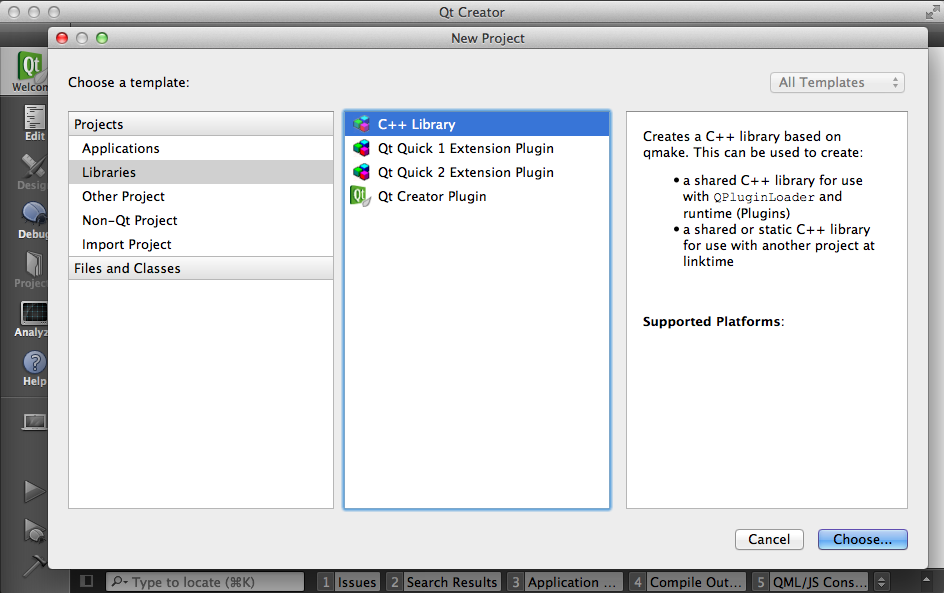
\includegraphics[width=\linewidth]{qt-creator}
 \caption{Zaslonska slika orodja Qt Creator.}
 \label{fig:qt-creator}
\end{figure}

Ogrodje Qt je primerno za izdelavo aplikacij, ki vključujejo kompleksne algoritme, za katere bi porabili preveč časa pri prilagajanju za različne platforme. Lep primer tega sta aplikaciji Mathematica\cite{mathematica} in multimedijski predvajalnik VLC\cite{vlc}.

Glavne slabosti Qt so neskladnost z izgledom ostalih aplikacij na mobilnih platformah, plačljiva licenca za razvoj mobilnih aplikacij ter končna velikost samih programov. Manjka tudi napovedana podpora za platformo Windows Phone.

\subsection{Xamarin}

Xamarin\cite{xamarin} je ogrodje za sočasen razvoj aplikacij za platforme iOS, Android, Mac in Windows v jeziku C\#. Izhaja iz projekta Mono\cite{mono}, ki omogoča uporabo ogrodja .NET\cite{dotnet} na različnih platformah. Ogrodje omogoča razvoj aplikacij, katerih izgled je skladen z ostalimi domorodnimi aplikacijami.

Ogrodje odlikuje integrirano razvojno okolje (\gls{ide}) Xamarin Studio (slika \ref{fig:xamarin}), ki razvoj aplikacij znatno olajša. Omogoča testiranje tako v emulatorju/simulatorju kot tudi na samih napravah.

\begin{figure}
 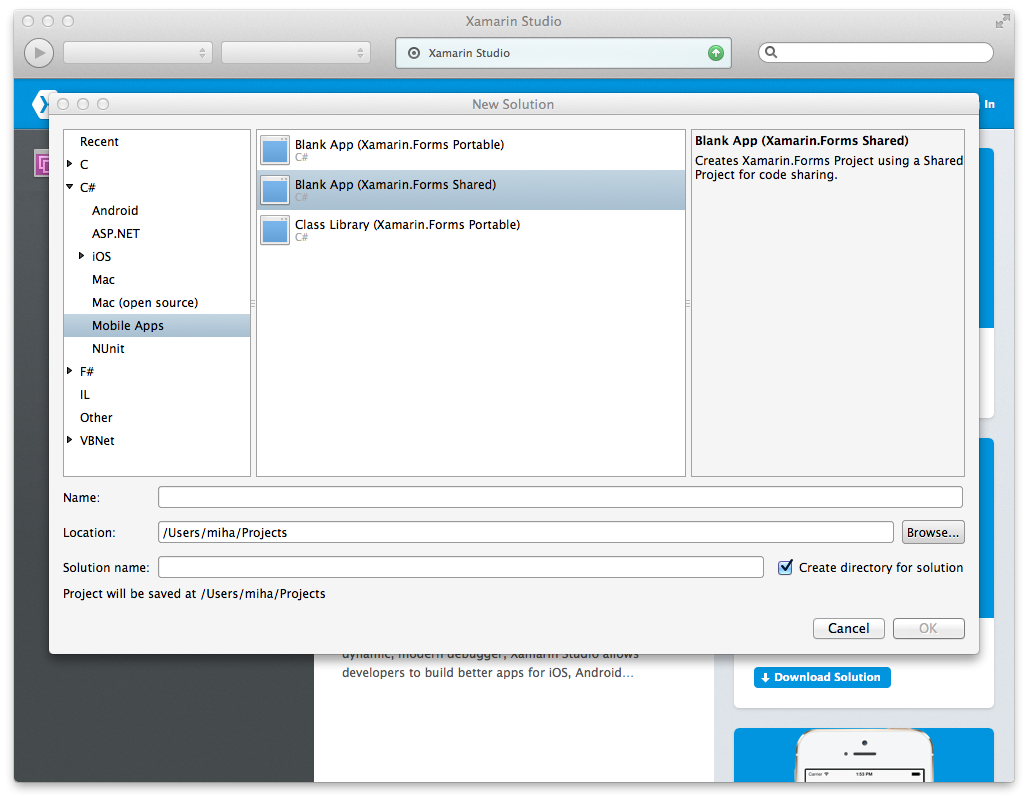
\includegraphics[width=\linewidth]{xamarin}
 \caption{Zaslonska slika orodja Xamarin Studio.}
 \label{fig:xamarin}
\end{figure}

Xamarin je primeren za izdelavo aplikacij za platforme, kjer je ključnega pomena končna grafična skladnost z ostalimi domorodnimi aplikacijami. Kot primer si lahko ogledamo aplikacijo za poslušanje glasbe Rdio\cite{rdio}, ki je na voljo za iOS, Android in Windows Phone.

Glavna slabost ogrodja Xamarin je cena, saj se paketi začnejo šele pri 299\$/mesec za vsakega razvijalca in vsako platformo posebej. Za majhno ekipo je lahko taka začetna cena enostavno previsoka. Vprašljiva je tudi hitrost dodajanja funkcionalnosti posameznih platform, ko se te nadgradijo, določeno tveganje predstavlja tudi muhavost posameznih platform pri omejitvah uporabe tega ogrodja, sploh če nadgradnja povzroči nedelovanje takih aplikacij.

\subsection{Adobe Air}

Adobe Air\cite{adobeair} je brezplačno ogrodje, ki omogoča zagon iste aplikacije na platformah iOS, Android, Mac, Windows in Linux, zagon aplikacije pa je možen tudi iz spletnega brskalnika. Čeprav za razvoj namiznih aplikacij omogoča uporabo HTML in Javascript, je razvoj mobilnih aplikacij omejen na uporabo jezika ActionScript. V času pisanja diplomske naloge ogrodje ne omogoča zagona na platformi Windows Phone, vendar so razvijalci podporo že napovedali.

Izbor orodja je še posebej uporaben za aplikacije, v katerih uporabniški vmesnik ni potrebno prilagajati posamezni platformi. Ravno zaradi tega je orodje priljubljeno med razvijalci iger, ko je na primer Angry Birds\cite{angrybirds}.

Kot glavno slabost ogrodja Adobe Air bi navedel upadanje zanimanja za orodje Flash. Špekuliramo lahko tudi o planih podjetja Adobe, saj so pred kratkim kupili podjetje Nitobi, ki je avtor ogrodja PhoneGap (katerega si bomo ogledali v nadaljevanju). Uporaba tudi ni primerna za razvoj klasičnih mobilnih aplikacij, saj je prilagajanje domorodnim aplikacijam precej zahtevno še posebej, kadar na platformi pride do posodobitve izgleda.

%-----
\section{Hibridne metode}

Hibridna metoda za razvoj aplikacij uporablja spletne tehnologije v sožitju z domorodno kodo za posamezno platformo (t.i. premostitvena tehnika), ki omogoča dostop do glavnih funkcij naprav (kot so kamera, pospeškomer in podobno). Tako kot pri celovitih metodah je tudi tu rezultat domorodna aplikacija, ki jo je možno objaviti v trgovinah posameznih platform.

\subsection{Apache Cordova / PhoneGap}

Ogrodje Apache Cordova\cite{cordova} je odprtokodni projekt, ki omogoča objavo spletnih aplikacij kot domorodne\cite{web-vs-native}. V času pisanja diplomske naloge ogrodje podpira iOS, Android, Windows Phone, Blackberry, Palm WebOS, Bada in Symbian. Na vseh omenjenih platformah nam ogrodje Apache Cordova omogoča dostop do funkcij naprave, ko so naprimer kamera in pospeškomer. Isto aplikacijo je možno zagnati tudi v spletnem brskalniku, a je za to potrebno nekaj dodatnega dela. Ogrodje Cordova je izdano pod odprtokodno licenco Apache 2.0\cite{apache-licence}.

Projekt PhoneGap\cite{phonegap} je dejansko samo ena od distribucij projekta Apache Cordova, ki poleg vseh obstoječih funkcionalnosti ponuja tudi razne storitve, na katerih delajo v podjetju Adobe. Vključuje tudi priročen program za ukazno vrstico, ki nam olajša delo s PhoneGap projektom (primer \ref{code:phonegap})

\begin{lstlisting}[caption=Primer uporabe programa phonegap za ukazno vrstico. Zadnja vrstica zažene pravkar ustvarjeno prazno aplikacijo na Android napravi ali emulatorju., label=code:phonegap]
$ phonegap create thesis
$ cd thesis
$ phonegap run android
\end{lstlisting}

Za razvoj aplikacij razvijalci lahko uporabljajo spletne tehnologije HTML, \gls{css} in JavaScript. S pomočjo ogrodij jQuery Mobile\cite{jquerymobile} in Sencha Touch\cite{sencha} je možno izdelati aplikacije, katerih izgled je zelo lep približek ostalim aplikacijam na izbrani platformi. Če naletimo na funkcijo naprave, do katere nimamo dostopa, ali ugotovimo, da je JavaScript za določene naloge premalo učinkovit, lahko preprosto spišemo lasten vtičnik (\eng{plugin}), ki služi kot most med kodo, napisano v jeziku JavaScript, in domorodno kodo.

Glavna prednost ogrodja Apache Cordova in predvsem distribucije PhoneGap je izredno velika nezahtevnost ogrodja. Priporoča se predvsem za izdelavo prototipnih aplikacij, saj nam omogoča hiter razvoj in iteracijo.

Glavna slabost tega pristopa tiči v performanci in odzivnosti aplikacije, saj le-ta za prikazovanje izkorišča vgrajeno spletno okno. Trenutno je težko izdelati aplikacije, ki so grafično zahtevnejše, kar predstavlja še toliko bolj pereč problem na napravah s slabšimi karakteristikami. Da se aplikacija po izgledu ne bi ločila od domorodnih aplikacij, je potrebno vložiti kar nekaj dela, na koncu pa bo izurjen uporabnik najbrž vseeno opazil, da je aplikacija malce drugačna. Problem predstavlja tudi zamik podpore novim stilom grafičnih elementov, tako kot se je to zgodilo pri prehodu z iOS6 na iOS7.

\subsection{Appcelerator Titanium}

Ogrodje Titanium\cite{titanium} nam omogoča izdelavo aplikacij za več platform hkrati s pomočjo JavaScript okolja, ki služi kot abstrakcijska plast med našo aplikacijo in domorodno kodo. Aplikacijo gradimo s pomočjo jezika JavaScript, ki se med uporabo aplikacije izvaja s pomočjo pogona V8\cite{v8} (Android), JavaScriptCore (iOS)\cite{javascriptcore} ali vgrajenega JavaScript okolja (če aplikacijo poganjamo v brskalniku). Za pravilen izgled skrbijo namestniški elementi, ki uporabljajo domorodne grafične elemente, kar pomeni, da aplikacije po izgledu ne moremo ločiti od ostalih domorodnih aplikacij. V času pisanja diplomske naloge ogrodje podpira iOS, Android, Blackberry, Tizen in spletne aplikacije. Tako kot PhoneGap je tudi Titanium na voljo pod odprtokodno licenco Apache 2.0. Za olajšanje razvoja so pri podjetju Appceletor razvili \gls{ide} Titanium Studio (slika \ref{fig:titanium-studio}), ki je prav tako na voljo brezplačno.

\begin{figure}
 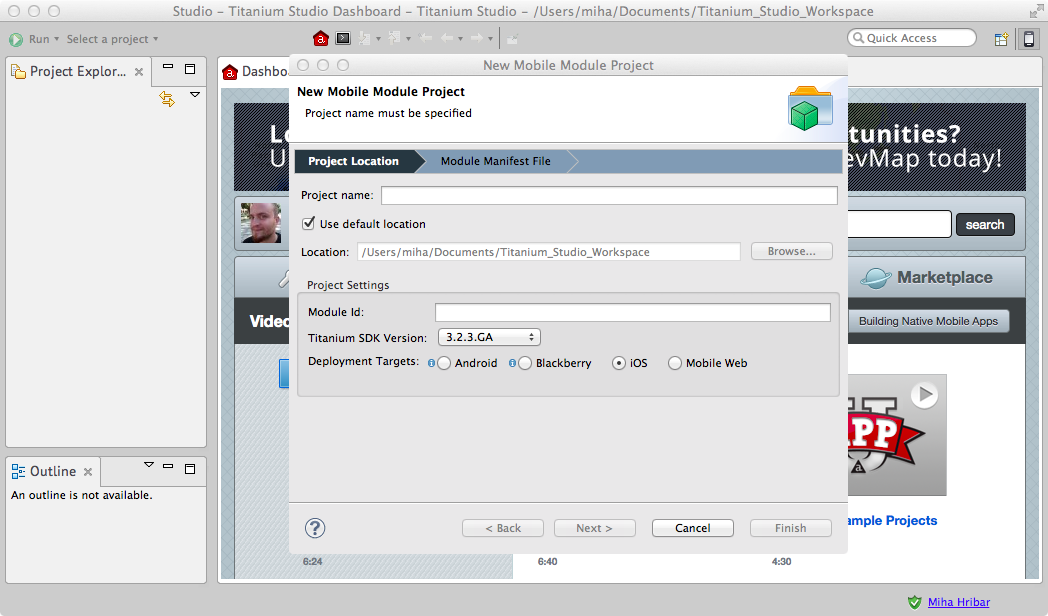
\includegraphics[width=\linewidth]{titanium}
 \caption{Zaslonska slika orodja IDE Titanium Studio.}
 \label{fig:titanium-studio}
\end{figure}

Glavna prednost ogrodja Titanium ni t.i. način ``piši enkrat, uporabljaj povsod'', temveč da lahko celotno aplikacijo izdelamo v enem jeziku - JavaScript-u. Le redko se bomo srečali z domorodno kodo, saj ogrodje nudi široko paleto knjižnic.

Tako kot PhoneGap je tudi Titanium še posebej uporaben pri razvoju prototipov aplikacij, kjer je cilj hiter razvoj in predstavitev aplikacije čim večjemu krogu uporabnikov.

Glavna slabost ogrodja je počasno dodajanje novih platform zaradi obsežnosti dela, ki ga tak podvig zahteva. Določene knjižnice za delo z domorodnimi elementi tudi niso najbolj performančne, manjka pa tudi napovedana podpora platformi Windows Phone.

%-----
\section{Deljene metode}

Deljena metoda za razvoj aplikacij omogoča uporabo dela aplikacijske kode na vseh platformah, za katere razvijamo. To lahko naredimo s pomočjo vgradnega skriptnega jezika (Lua), s pomočjo prevajanja iz izbranega programskega jezika v domorodnega (Haxe, XMLVM, Emscripten) ali pa z uporabo programskih jezikov C++ ali JavaScript in jezikovnih ovojev, s katerimi pripravimo knjižnico za vgradnjo v druge platforme.

\subsection{Lua}

Lua\cite{lua} je preprost vgradni skriptni jezik, ki ga odlikuje hitrost izvajanja in procesorska nezahtevnost. Vgradimo ga lahko v platforme Android, iOS, Symbian in Windows Phone, z nekaj potrpljenja pa lahko isto kodo zaženemo tudi v spletni aplikaciji. Lua je na voljo pod odprtokodno licenco MIT\cite{mit}.

Ker gre za skriptni jezik, se znajdemo v zanimiv situaciji, kjer združujemo prevajane jezike z interpretiranimi jeziki. Velika prednost tega je hitro odzivanje na napake pri razvoju, saj razvijalcu ni potrebno čakati na prevod kode. Odpira tudi možnost posodobitve vgrajene knjižnice brez posodobitve celotne aplikacije.

\begin{lstlisting}[caption={Primer metode v skriptnem jeziku Lua, ki datum iz oblike 2014-07-14 razbije na leto, mesec in dan.}, label=code:lua, language=LUA]
function get_date_parts(date_str)
  _,_,y,m,d=string.find(date_str, "(%d+)-(%d+)-(%d+)")
  return tonumber(y),tonumber(m),tonumber(d)
end
\end{lstlisting}

Čeprav je jezik Lua preprost za uporabo, se izkaže, da za kompleksnejše knjižnice ni primeren. Manjka podpora Unicode\footnote{Standard za poenoteno tekstovno enkodiranje.}, boljša podpora rokovanju z napakami, boljša podpora starejšim verzijam in vgrajen razhroščevalnik (\eng{debugger}).

\subsection{Haxe}

Haxe\cite{haxe} zase pravi, da je večplatformski programski jezik. Razvijalec lahko svojo aplikacijo napiše v jeziku Haxe, nato pa jo s pomočjo prevajalnika prevede v izvorno kodo jezikov \gls{php}, ActionScript, Neko, JavaScript, C++, C\# in Java. Nudi tudi dodatne vmesnike za dostop do specifičnih metod ciljnega jezika. Haxe prevajalnik je na voljo pod licenco \gls{gpl}, haxe knjižnice, ki jih potrebujemo za razvoj aplikacij, pa so na voljo pod licenco MIT.

Jezik se uporablja predvsem pri razvoju iger, kjer naj bi v prihodnosti zamenjal jezik ActionScript, ki ga uporablja orodje Flash.

Glavna slabost uporaba rešitve Haxe je majhna razvijalska skupnost. V primerjavi z ostalimi rešitvami je ta kar v manjšini. V zadnjem času sicer pridobiva nekaj zagona, a je trenutno vse premalo knjižnic, ki bi bile razvite za to platformo.

\subsection{XMLVM}

XMLVM\cite{xmlvm} spada v isti razred kot Haxe - tako imenovanih prevajalcev iz enega jezika v drugega (ang. cross-compilers) - a se XMLVM tega loti na drugačen način. Medtem ko Haxe prevaja na nivoju izvorne kode, XMLVM to počne na nivoju zlogovne kode (ang. byte code). Izvorna koda je lahko napisana za navidezne stroje (ang. virtual machine) \gls{jvm}, .NET \gls{cli} ali Ruby \gls{yarv}, medtem ko je rezultat delujoč program za JVM, .NET CLI, Javascript, Python, Objective-C in C++. Ogrodje je na voljo pod odprtokodno licenco \gls{lgpl}.

Projekt je bil zastavljen zelo ambiciozno, a vse kaže, da je šlo le za akademsko raziskavo. Od zadnje posodobitve izvorne kode je namreč minilo že več kot leto dni. Kljub temu se mi je projekt zdel zanimiv in ga je bilo vredno izpostaviti.

\subsection{C++ in Emscripten}

V kolikor nobena od naštetih možnosti ne zadošča našim potrebam, vseeno pa bi želeli imeti deljeno knjižnico, obstaja še ena možnost: uporaba jezika C++\cite{cpp} in projekta Emscripten\cite{emscripten}.

C++ je eden izmed najbolj razširjenih programskih jezikov. V času pisanja diplomske naloge zaseda četrto mesto na lestvici najbolj popularnih jezikov \ref{fig:tiobe-index}, pred njim so samo jeziki C, Java in Objective-C. Uporablja se ga v raznolikih projektih - od prevajalnikov, strežnikov do video igric.

\begin{figure}
 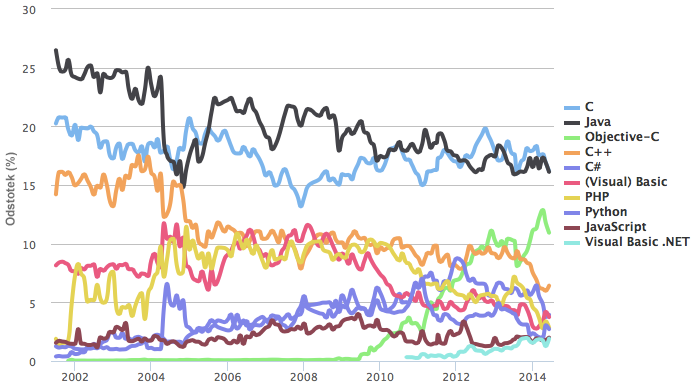
\includegraphics[width=\linewidth]{tiobe-index}
 \caption{Tiobe programming comunity index\cite{tiobe}.}
 \label{fig:tiobe-index}
\end{figure}

Emscripten je projekt Mozillinih laboratorijev, ki omogoča prevajanje iz \gls{llvm} zlogovne kode v skriptni jezik JavaScript. LLVM si lahko predstavljamo kot vmesni sloj med izvorno (C, C++, Objective-C, Java, C\#) in strojno kodo, ki poskrbi za visoko optimizacijo vmesne kode, to pa lahko potem prevedemo v ustrezen nabor ukazov za posamezne procesorje (\gls{arm}, x86 itd.). Emscripten tako predstavlja zadnjo fazo prevajalnika, le da vmesne kode iz LLVM ne prevede v ukaze specifičnega procesorja, ampak nazaj v jezik JavaScript. To pomeni, da lahko (z določenimi omejitvami) prevedemo skoraj vsak program v JavaScript in ga zaženemo v brskalniku. Celo grafično zahtevne aplikacije\footnote{Skupina Mozillinih inženirjev je grafično ogrodje Unreal v štirih dneh posodobilo do te mere, da je lahko s pomočjo orodja Emscripten grafično zahtevna aplikacija brezhibno delovala v brskalniku\cite{epic-citadel}.} niso problematične, saj Emscripten za prevod v JavaScript uporablja asm.js\cite{asmjs}, kar je podmnožica jezika JavaScript, ki jo JavaScript pogoni znajo izredno dobro optimizirati\footnote{S pomočjo asm.js so v podjetju Mozilla uspeli doseči le enkrat počasnejše izvajanje od domorodne kode, kar je izjemen dosežek.\cite{mozilla-asmjs}}.

\subsection{JavaScript}
\label{chap:javascript}

Namesto prevajanja v jezik JavaScript s pomočjo ogrodja Emscripten bi lahko celotno knjižnico napisali kar v jeziku JavaScript. V zadnjih nekaj letih je jezik JavaScript doživel izredno hitro rast tako v popularnosti kot tudi v zmogljivosti in funkcionalnostih, kar je tudi razvidno iz slike \ref{fig:github-jeziki}.

\begin{figure}
 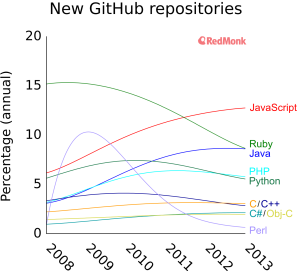
\includegraphics[width=\linewidth]{github-jeziki}
 \caption{Jeziki novih projektov na spletni strani github.com, povzeto po\cite{redmonk}}
 \label{fig:github-jeziki}
\end{figure}

Pri vključitvi v svojo aplikacijo moramo biti malce bolj iznajdljivi. iOS je z verzijo 7 dodal knjižnico JavaScriptCore\cite{javascriptcore-docs}, ki omogoča mešanje domorodne in JavaScript kode.

Android je malce bolj problematičen, saj njegov \gls{sdk} v času pisanja diplomske naloge ne nudi direktne implementacije. Zaradi tega smo primorani vključiti JavaScript pogon, kot so Rhino, V8 in podobni. V kolikor je pogon napisan v jeziku Java, je integracija preprosta, če pa izberemo pogon v drugem jeziku, mora za Android obstajati paket za uvoz.

Windows Phone prav tako kot Android ne nudi JavaScript implementacije, ki bi jo lahko uporabljali skupaj z domorodno kodo. Uporabimo lahko pogon V8 in knjižnico JavaScriptNet\cite{javascriptdotnet}.

Ker je knjižnica napisana v jeziku JavaScript, jo je možno preprosto vgraditi v spletno aplikacijo. Pri tem se moramo držati le delov JavaScripta, ki so enotni na vseh platformah (ECMAScript specifikacija\cite{ecmascript}).

Težji del je vgraditev pogona JavaScript na posamezno platformo. Dokler ne bo na voljo domorodnih integracij, se bomo težko zanesli na brezhibno delovanje pri nadgradnji operacijskega sistema. Kljub temu je ideja zelo zanimiva in vredna nadaljnje raziskave.

%==============================
\chapter{Razvoj knjižnice}
\label{chap:development}

%-----
\section{Uvod}

Izbor primerne metode si bomo pogledali na primeru razvoja koledarske aplikacije, ki bo tekla na platformah iOS, Android, Windows Phone in tudi v spletni aplikaciji. V aplikaciji bo uporabnik lahko dodal koledarski dogodek, ki mu bo možno nastaviti različne frekvence ponavljanj, intervale in izjeme. Aplikacija bo nato za določen datumski interval prikazala vnešeni dogodek v preprostem seznamu (slika \ref{fig:app-ios}).

\begin{figure}
 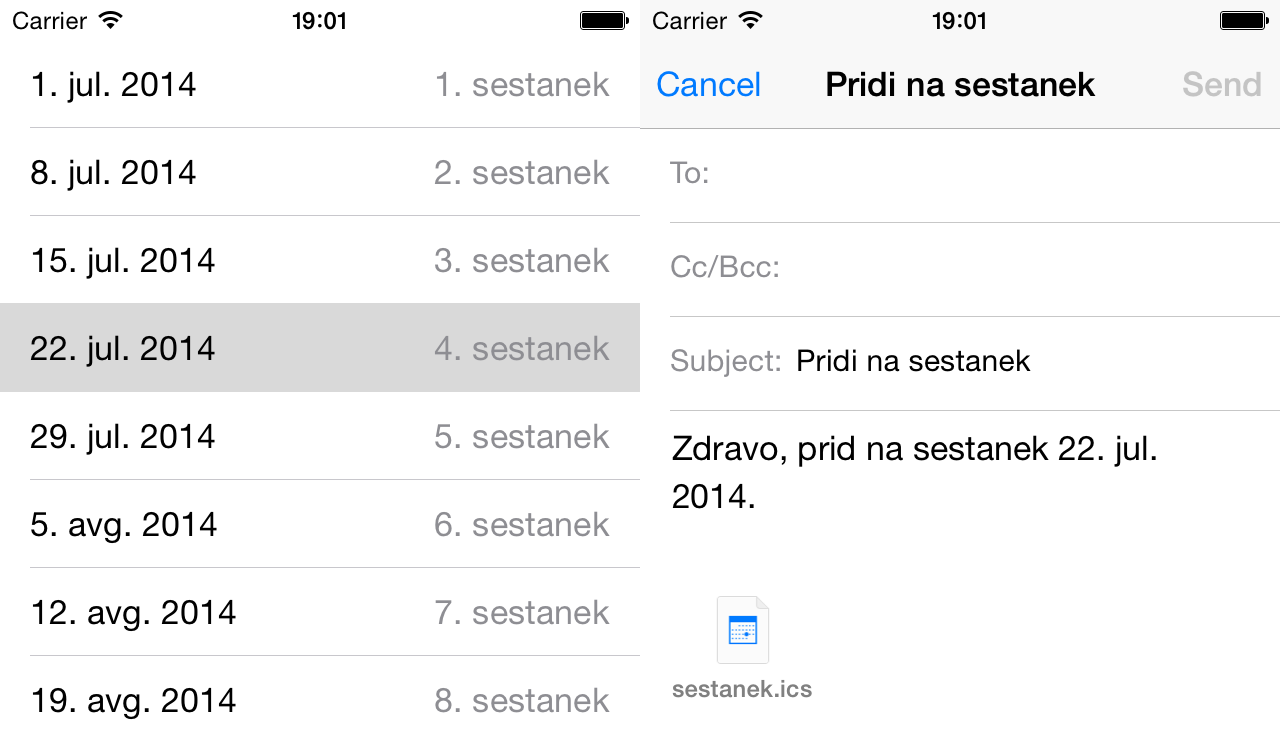
\includegraphics[width=\linewidth]{app-ios}
 \caption{Zaslonska slika dveh delov preproste koledarske aplikacije.}
 \label{fig:app-ios}
\end{figure}

Vnešeni dogodek bo uporabnik aplikacije lahko delil z ostalimi preko e-poštnega sporočila, ki bo vseboval format iCalendar, opisan v specifikaciji RFC 5545\cite{rfc5545}, ki si ga bomo podrobneje ogledali v naslednjem poglavju.

%-----
\section{Predstavitev specifikacije RFC 5545}

Specifikacija RFC 5545\cite{rfc5545} opisuje format iCalendar, ki se uporablja za dogovarjanje o urnikih sestankov in umeščanju na koledar. Gre za tekstovni format, katerega prepoznavna končnica datotek je \texttt{.ics}, in je dandanes v uporabi v vseh večjih koledarskih aplikacijah, kot so Google Calendar, Apple Calendar in ostale. Omogoča vse, kar potrebujemo za opisovanje dogodkov, med drugim:

\begin{itemize}
  \item Datum začetka in konca dogodka
  \item Nastavitve opozoril
  \item Opis in priponke
  \item Seznam povabljenih ljudi
  \item Pravila za ponavljanje dogodka
\end{itemize}

Zaradi obsežnosti specifikacije se bomo v diplomski nalogi osredotočili zgolj na pravila za ponavljanje dogodkov\cite{rrule}. Če primer \ref{code:rrule} prevedemo v človeku prijazno obliko, bi to pomenilo ``vsako nedeljo v januarju, ob 8:30 zjutraj in 9:30 zjutraj, vsako drugo leto''.

\begin{lstlisting}[caption=Primer uporabe pravila RRULE spefikiacije RFC 5545., label=code:rrule]
FREQ=YEARLY;INTERVAL=2;BYMONTH=1;BYDAY=SU;BYHOUR=8,9;BYMINUTE=30
\end{lstlisting}

Vsak del pravila sestavlja par, sestavljen iz imena pravila in vrednosti. Vsak par je med seboj ločen z podpičjem (;), vsako pravilo pa je lahko določeno le enkrat. Vrstni red načeloma ni pomemben, a zaradi združljivosti s starejšimi specifikacijami mora biti pravilo \texttt{FREQ} vedno na prvem mestu.

Pravilo \texttt{FREQ} predstavlja frekvenco ponavljanja dogodka. Možne vrednosti so:

\begin{itemize}
  \item \texttt{SECONDLY}, za ponavljanje vsako sekundo
  \item \texttt{MINUTELY}, za ponavljanje vsako minuto
  \item \texttt{HOURLY}, za ponavljanje vsako uro
  \item \texttt{DAILY}, za dnevno ponavljanje
  \item \texttt{WEEKLY}, za tedensko ponavljanje
  \item \texttt{MONTHLY}, za mesečno ponavljanje
  \item \texttt{YEARLY}, za letno ponavljanje
\end{itemize}

Pravilo \texttt{INTERVAL} vsebuje pozitivno celo število, ki predstavlja interval ponavljanja frekvence. Če je frekvenca nastavljena na dnevno, interval pa na 8, pomeni, da se dogodek ponovi vsak 8. dan.

Pravilo \texttt{UNTIL} definira končni datum ponavljanja dogodka (vključno s končnim datumom). Definiramo ga lahko samo z datumom ali pa z datumom in uro.

Pravilo \texttt{COUNT} vsebuje pozitivno celo število, ki predstavlja število ponovitev dogodka. V kolikor ima pravilo nastavljeno tako \texttt{UNTIL} kot \texttt{COUNT}, obvelja tisto pravilo, ki ponavljanje dogodka prej konča.

Pravila \texttt{BYSECOND}, \texttt{BYMINUTE} in \texttt{BYHOUR} vsebujejo z vejico ločene sezname pozitivnih celih števil. Možne vrednosti \texttt{BYSECOND} so od 0 do 60, \texttt{BYMINUTE} od 0 do 59 in \texttt{BYHOUR} od 0 do 23. Če nastavimo pravilo \texttt{BYHOUR} na vrednost \texttt{8,20}, se bo dogodek ponovil ob 8h zjutraj in 8h zvečer.

Pravilo \texttt{BYDAY} vsebuje z vejico ločen seznam dnevov v tednu, kjer je \texttt{MO} ponedeljek, \texttt{TU} torek, \texttt{WE} sreda, \texttt{TH} četrtek, \texttt{FR} petek, \texttt{SA} sobota in \texttt{SU} nedelja. Pred oznako za posamezen dan lahko postavimo pozitivno ali negativno celo število, ki predstavlja N-to ponovitev v mesečnem ali letnem ponavljanju dogodka. Za mesečno ponavljanje dogodka vrednost \texttt{+1MO} pomeni vsak prvi ponedeljek v mesecu, \texttt{-1MO} vsak zadnji ponedeljek v mesecu, \texttt{MO} pa preprosto vsak ponedeljek v mesecu.

Pravilo \texttt{BYMONTHDAY} vsebuje z vejico ločen seznam celih števil z možnimi vrednostmi od -31 do -1 in 1 do 31, ki prestavljajo dneve v mesecu. Vrednost \texttt{-10} predstavlja 10. dan od konca meseca. Pravilo \texttt{BYMONTHDAY} ne sme biti nastavljeno, če je frekvenca ponavljanja nastavljena na tedensko.

Pravilo \texttt{BYYEARDAY} vsebuje z vejico ločen seznam celih števil z možnimi vrednostmi od -366 do -1 in 1 do 366, ki predstavljajo dneve v letu. Vrednost \texttt{-1} predstavlja zadnji dan v letu (31. december), \texttt{-306} pa 306. dan od konca leta (1. marec). Pravilo \texttt{BYYEARDAY} ne sme biti uporabljeno, če je v uporabi dnevna, tedenska ali mesečna frekvenca ponavljanja dogodka.

Pravilo \texttt{BYWEEKNO} vsebuje z vejico ločen seznam celih števil z možnimi vrednostmi od -53 do -1 in 1 do 53, ki predstavljajo tedne v letu. Prvi teden v letu je tisti, ki ima vsaj 4 dni v koledarskem letu. Vrednost \texttt{3} predstavlja tretji teden v letu. Pravilo \texttt{BYWEEKNO} je lahko definirano le, če imamo opravka z letno frekvenco dogodka.

Pravilo \texttt{BYMONTH} vsebuje z vejico ločen seznam pozitivnih celih števil z možnimi vrednostmi od 1 do 12, ki predstavljajo mesece v letu. Vrednost \texttt{2} predstavlja 2. mesec v letu.

S pravilom \texttt{WKST} definiramo dan začetka tedna. Možne vrednosti so iste kot pri pravilu \texttt{BYDAY}. Vrednost \texttt{SU} pomeni, da se delovni teden za nas začne v nedeljo. Če pravilo ni posebej nastavljeno, obvelja vrednost \texttt{MO}.

Pravilo \texttt{BYSETPOS} vsebuje z vejico ločen seznam celih števil z možnimi vrednostmi od -366 do -1 in 1 do 366. Predstavljajo N-to ponovitev znotraj pravil \texttt{BYSECOND}, \texttt{BYMINUTE}, \texttt{BYHOUR}, \texttt{BYDAY}, \texttt{BYMONTHDAY}, \texttt{BYYEARDAY} in \texttt{BYWEEKNO}. Primer \ref{code:rrule-last-work-day} predstavlja zadnji delovni dan v mesecu.

\begin{lstlisting}[caption=Primer uporabe pravila za zadnji delovni dan v mesecu., label=code:rrule-last-work-day]
FREQ=MONTHLY;BYDAY=MO,TU,WE,TH,FR;BYSETPOS=-1
\end{lstlisting}

Pravila lahko v nekaterih situacijah povzročijo ponovitev dogodka na neobstoječ datum, kot je naprimer 30. februar. V takih primerih se ponovitev dogodka preskoči brez opozorila.

Začetni datum ponavljanja dogodka je definiran izven omenjenih pravil, in sicer v delu \texttt{DTSTART}. Datum prve ponovitve dogodka je vedno isti začetnemu datumu, ne glede na to, če je ta dan smiseln glede na opisana pravila ponavljanja.

Opisana pravila s predpono \texttt{BY} vedno na nek način spremenijo ponavljanje dogodka. Število dni lahko ta pravila omejijo kot v primeru \texttt{FREQ=DAILY;BYMONTH=1}, kjer dnevno ponavljanje omeji samo na mesec januar. Lahko pa jih tudi razširijo, kot v primeru \texttt{FREQ=YEARLY;BYMONTH=1,2}, kjer je enkratno letno ponavljanje razširjeno na ponovitev vsak januar in februar, vsako leto.

\begin{table}
\footnotesize
\scalebox{0.85}{
\begin{tabular}{ l | l | l | l | l | l | l | l }
  \hline
  				& SECONDLY	& MINUTELY	& HOURLY	& DAILY		& WEEKLY 	& MONTHLY 	& YEARLY	\\
  \hline
  BYMONTH 		& omeji 	& omeji 	& omeji 	& omeji 	& omeji 	& omeji 	& razširi 	\\
  BYWEEKNO		& - 		& -			& - 		& - 		& -			& - 		& razširi 	\\
  BYYEARDAY		& omeji 	& omeji 	& omeji 	& - 		& - 		& - 		& razširi 	\\
  BYMONTHDAY	& omeji 	& omeji 	& omeji 	& omeji 	& - 		& razširi 	& razširi 	\\
  BYDAY 		& omeji 	& omeji 	& omeji 	& omeji 	& razširi 	& izjema 1 	& izjema 2 	\\
  BYHOUR		& omeji 	& omeji 	& omeji 	& razširi 	& razširi 	& razširi 	& razširi 	\\
  BYMINUTE 		& omeji 	& omeji 	& razširi 	& razširi 	& razširi 	& razširi 	& razširi 	\\
  BYSECOND 		& omeji 	& razširi 	& razširi 	& razširi 	& razširi 	& razširi 	& razširi 	\\
  BYSETPOS 		& omeji 	& omeji 	& omeji 	& omeji 	& omeji 	& omeji 	& omeji 	\\
  \hline
\end{tabular}}
\caption{Razpredelnica izjem pri uporabi pravil za ponavljanje dogodkov. \textbf{Izjema 1:} omeji, če je prisotno pravilo \texttt{BYMONTHDAY}, drugače razširi. \textbf{Izjema 2:} omeji za pravili \texttt{BYYEARDAY} in \texttt{BYMONTHDAY}, drugače razširi. }
\label{table:rrule-behavior}
\end{table}

Če je v pravilu ponavljanja uporabljenih več pravil s predpono \texttt{BY}, se ta obravnavajo v vrstnem redu \texttt{FREQ}, \texttt{INTERVAL}, \texttt{BYMONTH}, \texttt{BYWEEKNO}, \texttt{BYYEARDAY}, \texttt{BYMONTHDAY}, \texttt{BYDAY}, \texttt{BYHOUR}, \texttt{BYMINUTE}, \texttt{BYSECOND}, \texttt{BYSETPOS}, \texttt{COUNT} in \texttt{UNTIL}.

Tabela \ref{table:rrule-behavior} opisuje vse izjeme, ki jih lahko povzročijo pravila s predpono \texttt{BY}.

%-----
\section{Omejitve}

Preden se lotimo izbora primerne metode, postavimo nekaj omejitev:

\begin{enumerate}
  \item Delovati mora na platformah iOS, Android, Windows Phone in spletu.
  \item Zagotavljati grafično skladnost z ostalimi domorodnimi aplikacijami.
  \item Imeti dovolj razgibano razvijalsko skupnost, da bomo lahko našli odgovore na nastale probleme.
  \item Mora biti odporna na spremembe pri nadgradnjah platforme.
  \item Biti cenovno ugodna.
\end{enumerate}

%-----
\section{Izbor primerne metode}

Izbor primerne metode lahko začnemo s pregledom popularnih vprašanj na spletni strani Stackoverflow (slika \ref{fig:stackoverflow-trends}). Vidimo lahko izjemno popularnost ogrodij Qt in PhoneGap. Kot opombo lahko omenim, da Xamarin na tem grafu ni prikazan zaradi premajhnega števila vprašanj. Prav tako ne bi bilo ravno smiselno vključiti jezik C++ ali JavaScript, saj ti podatki ne bi bili reprezentativni.

\begin{figure}
 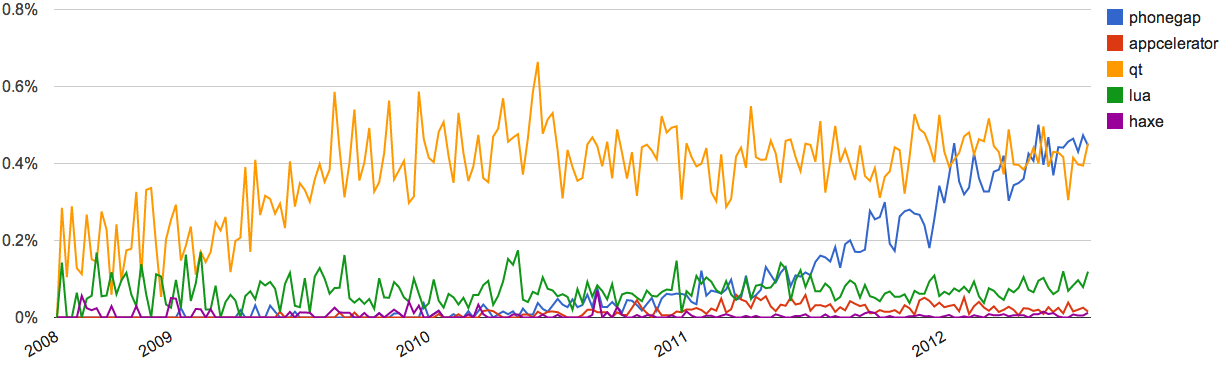
\includegraphics[width=\linewidth]{stackoverflow-trends}
 \caption{Prikaz procenta tedenskih trendov vprašanj za nekaj od predlaganih rešitev na spletni strani Stackoverflow, kjer razvijalci iščejo rešitve problemov, na katere so naleteli.}
 \label{fig:stackoverflow-trends}
\end{figure}

Vse omejitve, omenjene v prejšnjem poglavju, so predstavljene v tabeli \ref{table:omejitve}. Prazne vrstice pri ``grafični skladnosti'' za Lua, Haxe, C++ in JavaScript so posledica nezmožnosti zadostitvi tem omejitvam, niso pa ovira, saj mora v tem primeru za grafično skladnost poskrbeti domorodna koda, ki ni napisana v omenjenih jezikih.

Iz tabele \ref{table:omejitve} je lepo razvidno, da le rešitev C++ zadošča vsem naštetim omejitvam. Namesto razvoja medplatformne aplikacije se bomo rajši odločili za razvoj medplatformne knjižnice, ki jo bomo nato vključili v domorodne aplikacije s pomočjo jezikovnih ovojev.

\begin{table}
\footnotesize
\scalebox{0.85}{
\begin{tabular}{ l | c | c | c | c | c | c | c | c | c }
  \hline
  							& Qt & Xamarin & Air & Cordova & Titanium & Lua & Haxe & C++ & JavaScript \\
  \hline
  Android 					& \cmark & \cmark & \cmark & \cmark & \cmark & \cmark & \cmark & \cmark & \cmark \\
  iOS 						& \cmark & \cmark & \cmark & \cmark & \cmark & \cmark & \cmark & \cmark & \cmark \\
  Windows Phone 			& \xmark & \cmark & \xmark & \cmark & \xmark & \cmark & \cmark & \cmark & \cmark \\
  Spletna aplikacija 		& \xmark & \xmark & \cmark & \cmark & \xmark & \cmark & \cmark & \cmark & \cmark \\
  Grafična skladnost 		& \xmark & \cmark & \xmark & \xmark & \cmark &        &        &        &        \\
  Skupnost 					& \cmark & \cmark & \xmark & \cmark & \cmark & \cmark & \xmark & \cmark & \cmark \\
  Odpornost na nadgradnje 	& \xmark & \xmark & \xmark & \xmark & \xmark & \xmark & \xmark & \cmark & \xmark \\
  Cena (mesečno) 			& 149\$  & 299\$  & -      & -      & -      & -      & -      & -      & -      \\
  \hline
\end{tabular}}
\caption{Pregled funkcionalnosti predstavljenih metod.}
\label{table:omejitve}
\end{table}

%-----
\section{C++}

Namesto razvoja lastne knjižnice bi lahko na tem mestu v naš projekt vključili odprtokodno knjižnico \texttt{libical}\cite{libical}, a bomo za potrebe diplomske naloge rajši izbrali samostojno rešitev, saj bomo s tem lahko podrobneje raziskali, kaj vse je potrebno za razvoj podobne knjižnice.

Izbrani del RRULE specifikacije RFC 5545 je na srečo dovolj preprost, da za razvoj potrebujemo le knjižnico \gls{stl}. V kolikor bi naša rešitev zahtevala vključitev dodatne knjižnice - recimo vzpostavitev internetne povezave - bi lahko ta problem rešili na dva načina:

\begin{enumerate}
  \item V našo rešitev bi vključili dodatno knjižnico \texttt{libcurl}. To bi povzročilo kar nekaj problemov pri vključevanju knjižnice na različnih platformah, saj bi morali knjižnico \texttt{libcurl} pripraviti za vsako platformo posebej.
  \item Nalogo vzpostavitve in prenosa podatkov iz oddaljene lokacije bi lahko delegirali v domorodno kodo, ki bi po končanju prenosa rezultat vrnila v našo knjižnico.
\end{enumerate}

Če izberemo prvi način, bo naša knjižnica podvajala funkcionalnost, ki že obstaja v domorodni kodi. Veliko lepša rešitev je uporaba delegiranja v domorodno kodo, saj lahko ta bolje izkorišča vse sposobnosti naprave. To sicer pomeni nekaj več kode v ovojih naše knjižnice (kar si bomo ogledali v poglavju \ref{chap:cross-platform}), a omogoča boljšo odpornost na nadgradnje operacijskega sistema ciljne platforme.

Razvito knjižnico lahko v aplikacije za različne platforme vključimo na več načinov:

\begin{enumerate}
  \item Z izvorno kodo C++, ki jo ciljni program vključi v svoj paket.
  \item Statično knjižnico (\eng{static library}), ki jo ciljni program vključi v svoj paket.
  \item Deljeno knjižnico (\eng{shared library}), ki jo ciljni program samo referencira, a je ne vključi neposredno v svoj paket.
\end{enumerate}

Pri vseh naštetih načinih je potrebna dodatna ovojna koda (\eng{wrapper}), ki je različna za vsako ciljno platformo. Podrobnosti teh ovojev si bomo ogledali v poglavju \ref{chap:cross-platform}.

Celotna izvorna koda knjižnice (skupaj z jezikovnimi ovoji) je na voljo na spletni strani \href{https://github.com/mihahribar/thesis}{github.com/mihahribar/thesis}. Zaradi zagotavljanja kakovosti (\eng{quality assurance}) je bila knjižnica razvita s testno usmerjenim razvojem \gls{tdd}\cite{tdd-cpp}. Za implementacijo testov sta bili uporabljeni izvrstni knjižnici \texttt{googletest}\cite{googletest} in \texttt{googlemock}\cite{googlemock}, knjižnica pa se lahko pohvali z več kot 90\% testno pokritostjo kode (\eng{code coverage}), kar je moč preveriti s pomočjo programa \texttt{gcov}.

\begin{figure}
 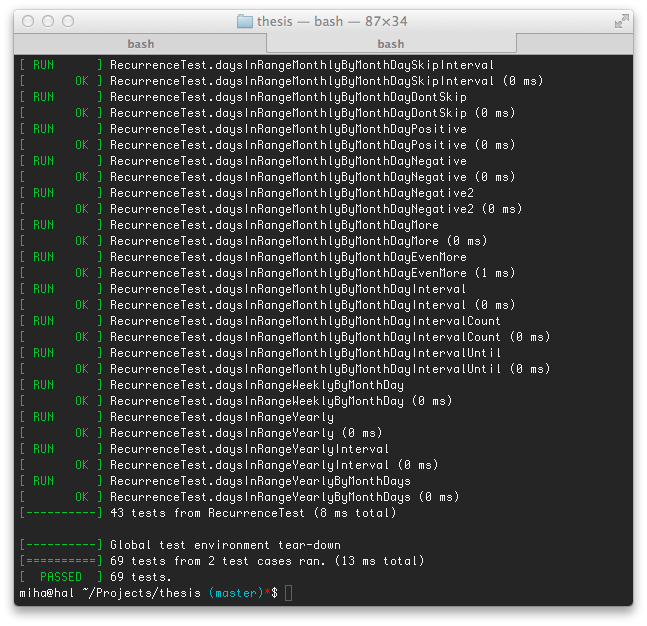
\includegraphics[width=\linewidth]{cpp-tests}
 \caption{Zaslonska slika testov C++ knjižnice.}
 \label{fig:cpp-tests}
\end{figure}

Za potrebe zvezne integracije (\eng{continuous integration}) projekt uporablja storitev Travis \gls{ci}\cite{travisci}, ki za odprtokodne projekte nudi brezplačno avtomatizirano testiranje. Vse, kar je potrebno storiti, da Travis CI lahko testira izvorno kodo knjižnice, je zapisano v datoteki \texttt{.travis.yml}. Ta vsebuje ukaz za zagon testov knjižnice (v našem primeru \texttt{make tests}), kar na strežniku za zvezno integracijo sproži prenos in pripravo knjižnic \texttt{googletest} in \texttt{googlemock}, prevede vse potrebne datoteke z izvorno kodo ter zgradi testni program, ki zažene vse naše testne primere.

\begin{lstlisting}[caption={Primer uporabe C++ knjižnice RRULE standarda RFC 5545. Izbrani dogodek bi se s tem pravilom ponavljal tedensko, vsak ponedeljek, od 1. januarja 2014 naprej.}, label=code:cpp-primer, language=C++]
Recurrence rec = Recurrence(Weekly, Date(2014, 1, 1));
rec.setByDay("MO");
map<int, Date> days = rec.daysInRange(Date(2014, 2, 1), Date(2014, 2, 28));
// spremenljivka days bo vsebovala
// result[5] = Date(2014, 2, 3);
// result[6] = Date(2014, 2, 10);
// result[7] = Date(2014, 2, 17);
// result[8] = Date(2014, 2, 24);
\end{lstlisting}

Primer uporabe knjižnice RRULE RFC 5545 lahko vidimo v primeru \ref{code:cpp-primer}. Razred \texttt{Date} vsebuje vso potrebno logiko za delo z datumi, kot so naprimer prištevanje, odštevanje ter primerjanje datumov. Razred \texttt{Recurrence} vsebuje logiko za ponavljanje dogodkov. Tip dogodka, ki se ponavlja, je poljuben in ni del knjižnice.

%==============================
\chapter[Vključitev knjižnice v različne platforme]{Vključitev knjižnice v \\ različne platforme}
\label{chap:cross-platform}

%-----
\section{iOS}

Platforma iOS primarno uporablja jezik Objective-C, ki je objektna razširitev jezika C. Na srečo obstaja tudi variacija Objective-C++, ki nam omogoča souporabo jezikov Objective-C in C++ v istem projektu. Datoteki, v kateri želimo uporabljati C++, namesto končnice \texttt{.m} pripnemo končnico \texttt{.mm}.

iOS ne podpira uporabe deljene knjižnice (\eng{shared library}), omogoča pa uporabo statične knjižnice (\eng{static library}) ali izvorne kode. Za prvi primer izberimo uvoz izvorne kode.

iOS v svojem arzenalu ne vključuje orodja za avtomatično sproščanje pomnilnika (\eng{garbage collection}). Od razvijalca se pričakuje, da za seboj počisti pomnilnik z uravnoteženimi ukazi \texttt{retain} in \texttt{release}, ko je koda opravila svoje delo. V ta namen je v integriranem razvijalskem okolju (\eng{Integrated Development Environment}) XCode na voljo kar nekaj orodij, ki nam omogočajo lažjo detekcijo puščanja pomnilnika (\eng{memory leak}). Kar rado se zgodi, da se pri štetju referenc razvijalec zmoti. Na srečo je v iOS5 Apple predstavil \gls{arc} (avtomatično štetje referenc - \eng{Automatic Reference Counting}), s čimer so razvijalcem znatno olajšali delo, saj prevajalnik sedaj sam zna vnesti ukaze za sproščanje pomnilnika.

Implementacija iOS ovoja je dokaj preprosta (glej primer \ref{code:ios-wrapper}). Za vsakega C++ od razredov naredimo zrcalne Objective-C++ ovojne razrede, ki v inicializacijski metodi \texttt{init} poskrbijo za pravilno dodeljevanje in hranjenje C++ objekta (vrstica 14). Ko na določen objekt ne kaže več noben kazalec, se pred sprostitvijo pomnilnika pokliče metoda \texttt{dealloc}, v kateri poskrbimo za ustrezno sprostitev C++ objekta, preden pride do puščanja pomnilnika (vrstica 21). Klic v ovoj nato preprosto posreduje klic v C++ objekt (vrstica 25) in poskrbi za transformacije med C++ in Objective-C podatkovnimi tipi.

\lstset{language=[Objective]C, breaklines}
\begin{lstlisting}[caption={Primer Objective-C++ ovoja C++ razreda \texttt{Date}.}, label=code:ios-wrapper]
#import "ThesisDate.h"
#import "Date.hpp"

@interface ThesisDate() {
    Thesis::Date* wrapped;
}
@end

@implementation ThesisDate

- (ThesisDate *)initWithYear:(NSInteger)year month:(NSInteger)month andDay:(NSInteger)day {
    self = [super init];
    if (self) {
        wrapped = new Thesis::Date(year, month, day);
        if (!wrapped) self = nil;
    }
    return self;
}

- (void)dealloc {
    delete wrapped;
}

- (void)addDays:(NSInteger)days {
    wrapped->addDays(days);
}
\end{lstlisting}

Razvojno okolje XCode vsebuje testno ogrodje \texttt{XCTest}, ki nam omogoča zagotavljanje kakovosti. Testi iOS ovoja testirajo samo klice v in povratne vrednosti, ne testirajo pa dejanske funkcionalnosti knjižnice, saj bi to pomenilo podvajanje že obstoječih testov C++ knjižnice. Teste zaženemo iz menija Product $\rightarrow$ Test.

\begin{figure}
 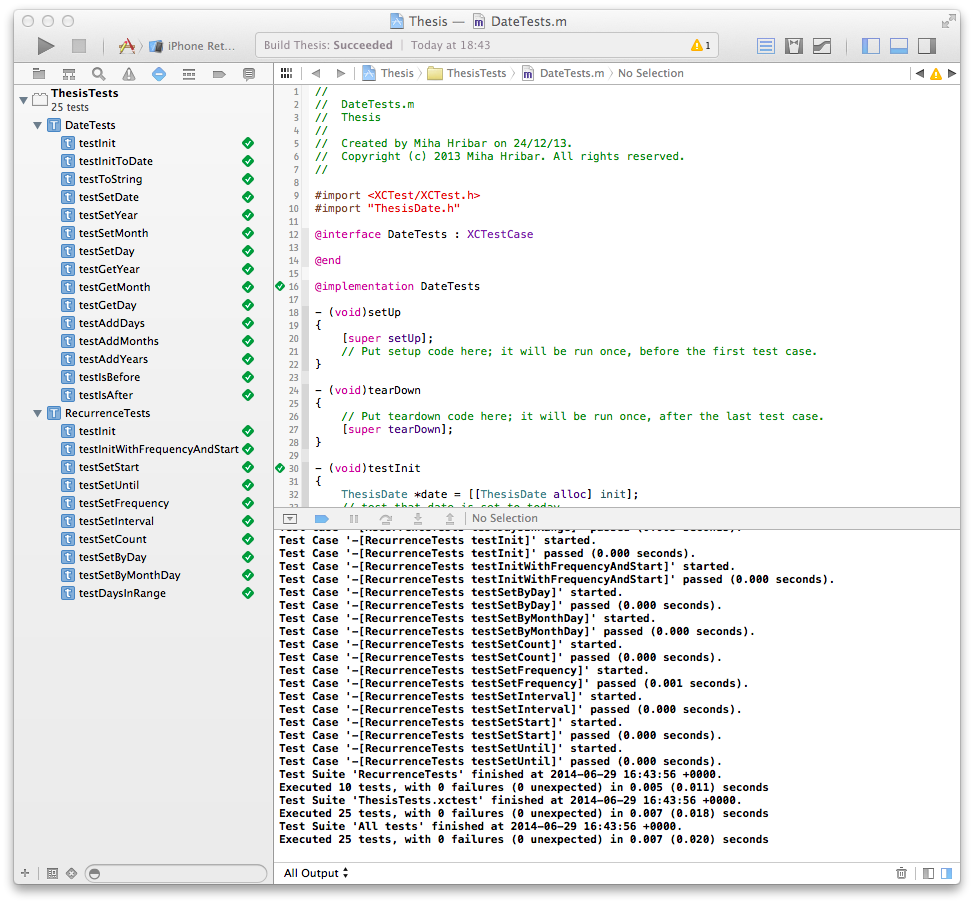
\includegraphics[width=\linewidth]{xcode-tests}
 \caption{Zaslonska slika zagona testov iOS ovoja C++ knjižnice v razvojnem okolju XCode.}
 \label{fig:xcode-tests}
\end{figure}

%-----
\section{Android}

Java, ki jo srečamo na platformi Android, se od odprtokodne Jave kar precej razlikuje. Android ne uporablja Java virtualnega pogona (\eng{Java Virtual Machine}), ampak svoj pogon Dalvik, ki je prilagojen za uporabo na mobilnih napravah. Pred kratkim je Google napovedal nov virtualen pogon, Android Runtime (\gls{art}), ki bo v prihodnosti zamenjal Dalvik in vsebuje veliko izboljšav v hitrosti in stabilnosti izvajanja aplikacij.

Za izdelavo ovoja C++ kode moramo uporabiti dve ogrodji:

\begin{enumerate}
  \item \gls{jni} (\eng{Java Native Interface}), ki poskrbi za komunikacijo med jezikoma Java in C++
  \item \gls{ndk} (\eng{Native Development Kit}), ki poskrbi za pravilno prevajanje C++ kode za vsako od ciljnih arhitektur Android platforme (armeabi, armeabi-v7a, x86 in mips).
\end{enumerate}

Uporaba ogrodja \gls{jni}\cite{jni-docs} je za razvijalca časovno kar potratna. Ovoj je potrebno napisati v dveh delih:

\begin{enumerate}
  \item Java ovoj, ki izpostavi C++ razrede in metode s pomočjo direktive \texttt{native} (glej primer \ref{code:android-java-wrapper}).
  \item C++ ovoj, ki služi kot most med jezikoma Java in C++ ter poskrbi za transformacije med podatkovnimi tipi (glej primer \ref{code:android-cpp-wrapper}).
\end{enumerate}

Referenco na C++ objekt hranimo v Java delu JNI ovoja, C++ ovoj pa do reference dostopa preko metode \texttt{getHandle} (glej \ref{code:android-cpp-wrapper}), ki spremenljivko \texttt{nativeHandle} poišče v Java delu JNI ovoja.

\begin{lstlisting}[caption={Primer Java ovoja C++ razreda \texttt{Date}.}, label=code:android-java-wrapper, language=Java]
public class Date
{
	private long nativeHandle = 0;
	public native void init(int year, int month, int day);
	public native boolean isBefore(Date date);
	public native void dispose();

	public Date(int year, int month, int day) {
		init(year, month, day);
	}

	static {
		System.loadLibrary("thesis");
	}
}
\end{lstlisting}

Java ovoje shranimo v direktorij \texttt{src}, medtem ko C++ JNI ovoje shranimo v \texttt{jni}. Poglejmo si, kako poteka komunikacija med Javo in C++ v primeru klica \texttt{isBefore} (glej primer \ref{code:android-cpp-wrapper}):

\begin{enumerate}
  \item Java preko JNI najde pravo metodo v C++ ovoju s pomočjo dogovorjene poimenovalne sheme (vrstica 12)
  \item C++ ovoj pretvori Java argumente v C++ argumente (vrstica 14).
  \item C++ ovoj najde predhodno shranjen objekt (vrstice 40-44).
  \item Pokliče pravilno metodo na najdenem objektu s C++ argumenti (vrstice 21-29).
  \item Če metoda vrne kak rezultat, C++ ovoj poskrbi za pretvorbo nazaj v Java podatkovne tipe (vrstica 13).
\end{enumerate}

\begin{lstlisting}[caption={Primer mosta med jezikoma Java in C++ razreda \texttt{Date}.}, label=code:android-cpp-wrapper, language=C++]
#include "info_hribar_thesis_Date.h"
#include "Date.cpp"

using namespace Thesis;

JNIEXPORT void JNICALL Java_info_hribar_thesis_Date_init(JNIEnv *env, jobject obj, jint year, jint month, jint day) {
	Date *date = new Date(year, month, day);
	setHandle(env, obj, date);
}

JNIEXPORT jboolean JNICALL Java_info_hribar_thesis_Date_isBefore(JNIEnv *env, jobject obj, jobject compare) {
	Date *date = getHandle<Date>(env, obj);
	return date->isBefore(getDate(env, compare));
}

JNIEXPORT void JNICALL Java_info_hribar_thesis_Date_dispose(JNIEnv *env, jobject obj) {
	Date *date = getHandle<Date>(env, obj);
	delete date;
}

Date getDate(JNIEnv *env, jobject date) {
	jclass dateCls = env->GetObjectClass(date);
	jmethodID mGetYear = env->GetMethodID(dateCls, "getYear", "()I");
	jmethodID mGetMonth = env->GetMethodID(dateCls, "getMonth", "()I");
	jmethodID mGetDay = env->GetMethodID(dateCls, "getDay", "()I");
	jint year = env->CallIntMethod(date, mGetYear);
	jint month = env->CallIntMethod(date, mGetMonth);
	jint day = env->CallIntMethod(date, mGetDay);
	return Date(year, month, day);
}

jfieldID getHandleField(JNIEnv *env, jobject obj)
{
    jclass c = env->GetObjectClass(obj);
    // J is the type signature for long:
    return env->GetFieldID(c, "nativeHandle", "J");
}

template <typename T>
T *getHandle(JNIEnv *env, jobject obj)
{
    jlong handle = env->GetLongField(obj, getHandleField(env, obj));
    return reinterpret_cast<T *>(handle);
}

template <typename T>
void setHandle(JNIEnv *env, jobject obj, T *t)
{
    jlong handle = reinterpret_cast<jlong>(t);
    env->SetLongField(obj, getHandleField(env, obj), handle);
}
\end{lstlisting}

Bralca morda zanima, čemu služi metoda \texttt{dispose} (vrstice 16-19). Java nam nudi avtomatično sproščanje pomnilnika (\eng{garbage collection}), medtem ko C++ od razvijalca zahteva samostojno čiščenje pomnilniških naslovov, ki niso več v uporabi. Ko v Javi pride do sproščanja pomnilnika, se pokliče metoda \texttt{finalize}, a kot lahko preberemo v dokumentaciji\cite{android-object}, do klica ne prihaja prav pogosto in se za tako uporabo ne priporoča. Poleg tega je vsak razred, ki implementira metodo \texttt{finalize}, deležen malce večje obdelave s strani operacijskega sistema, kar botruje počasnejšemu izvajanju. Ker želimo biti malce bolj prijazni do platforme, na kateri gostujemo, se držimo pravila: ko objekta ne potrebujemo več, ga sprostimo s pomočjo klica \texttt{dispose} (naprimer v \texttt{finally} \texttt{try catch finally} konstruktu).

Za testiranje Java ovoja smo uporabili ogrodji JUnit\cite{junit} in Maven\cite{maven}. Tako kot v primeru iOS ovoja se na tem mestu ne testira dejanske knjižnice, ampak zgolj povezavo iz C++ knjižnice v Java kodo. Teste lahko zaženemo z ukazom \texttt{mvn test}, ki s pomočjo orodja Maven poskrbi za prenos vseh potrebnih knjižnic in za zagon testov Java ovoja.

\begin{figure}
 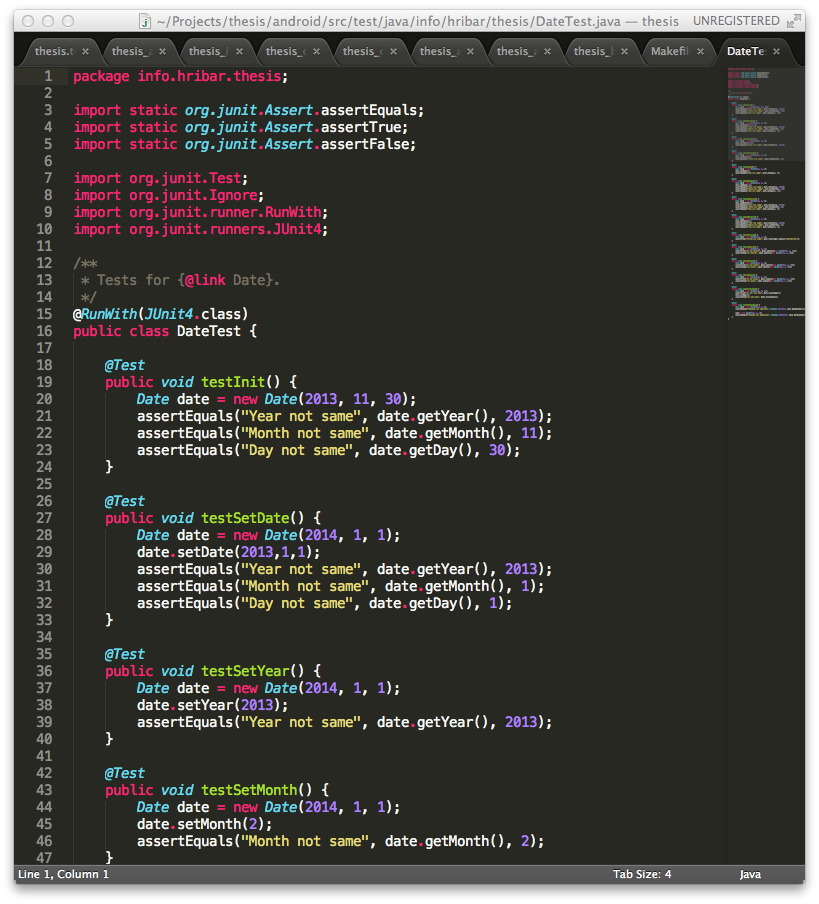
\includegraphics[width=\linewidth]{java-tests}
 \caption{Zaslonska slika, ki prikazuje teste razreda \texttt{Date} Java ovoja.}
 \label{fig:java-tests}
\end{figure}

%-----
\section{Windows Phone}

Primarni jezik vseh Windows platform je C\# in isto velja tudi za Windows Phone. Z 8. verzijo mobilnega operacijskega sistema je Microsoft odprl možnost souporabe C\# in domorodne kode. To storimo z uporabo Windows Phone Runtime komponente (WinPRT), ki jo spišemo v jeziku C++ in nato uvozimo v naš Windows Phone projekt kot zunanjo referenco.

Našo knjižnico lahko uvozimo kot statično knjižnico (\eng{static library}) ali direktno kot C++ izvorno kodo (če imamo do nje dostop). Če se odločimo za uporabo statične knjižnice, moramo paziti, da ta uporablja le standardno knjižnjico (\gls{stl}) in Win32 klice, ki so dovoljeni za Windows Phone aplikacije\cite{windows-static}.

Funkcionalnost, ki jo rabimo v naši Windows Phone 8 aplikaciji, izvozimo v WinPRT C++ komponenti (glej primer \ref{code:wp8-wrapper}).

\lstset{language=[Sharp]C, breaklines}
\begin{lstlisting}[caption={C++ koda za izvoz funkcionalnosti knjižnice v JavaScript razreda \texttt{Date}.}, label=code:wp8-wrapper, language=c++]
namespace ThesisWINRT {
    using namespace Windows::Foundation;
    using Platform::String;

    public ref class Date sealed {
    public:
        unsigned int GetLength(String^ strToParse);
    };
}
\end{lstlisting}

%-----
\section{Spletna aplikacija}

C++ knjižnico moramo za uporabo v spletni aplikaciji prevesti v JavaScript. To lahko storimo s pomočjo ogrodja Emscripten, ki vzame LLVM zlogovno kodo in namesto prevoda v nabor ukazov za podprte procesorje prevede to kodo v JavaScript. Rezultat je knjižnica, ki jo lahko brez težav uvozimo v obstoječo spletno aplikacijo.

Primarno Emscripten prevaja celotne programe, ki imajo jasno definirane vhode in izhode. Te lahko v JavaScriptu sprožimo, kot bi jih v uporabniški vrstici (\eng{terminal}). V našem primeru gre vendarle za prevod C++ knjižnice, za kar Emscripten potrebuje dodatna navodila za izvoz funkcionalnosti (glej primer \ref{code:emscripten-bindings}). Za te namene projekt Emscripten vsebuje \texttt{embind}\cite{emscripten-embind}, s pomočjo katerega lahko izvozimo dostop do razredov, podatkovnih tipov, pomnilniškim upravljanje in podobne jezikovne konstrukte.

\begin{lstlisting}[caption={C++ koda za izvoz funckionalnosti knjižnice v JavaScript razreda \texttt{Date}.}, label=code:emscripten-bindings, language=c++]
#include "emscripten/bind.h"
#include "src/Date.hpp"

using namespace emscripten;
using namespace Thesis;

EMSCRIPTEN_BINDINGS(date) {
    class_<Date>("Date")
        .constructor<int, int, int>()
        .property("year", &Date::getYear, &Date::setYear)
        .property("month", &Date::getMonth, &Date::setMonth)
        .property("day", &Date::getDay, &Date::setDay)
        .function("setDate", &Date::setDate)
        .function("addDays", &Date::addDays)
        .function("addMonths", &Date::addMonths)
        .function("addYears", &Date::addYears)
        .function("toString", &Date::toString)
        .function("isBefore", &Date::isBefore)
        .function("isAfter", &Date::isAfter)
        .function("isEqual", &Date::isEqual)
        .function("getWeekday", &Date::getWeekday)
        .function("isLastDay", &Date::isLastDay);
}
\end{lstlisting}

Končni rezultat izvoza knjižnice v JavaScript lahko vidimo v primeru \ref{code:javascript-date}.

\begin{lstlisting}[caption={Primer uporabe izvoženega razreda \texttt{Date} v JavaScript.}, label=code:javascript-date, language=JavaScript]
var date = new Thesis.Date(2014, 10, 10);
date.addMonths(1);
console.log(date.toString());
\end{lstlisting}


%==============================
\chapter{Evaluacija}
\label{chap:evaluation}

%-----
\section{Pregled prednosti, slabosti, priložnosti in nevarnosti}

Pred zaključnimi ugotovitvami si poglejmo prednosti, slabosti, priložnosti in nevarnosti (t.i \gls{swot} analiza) izbrane metode.

\subsection{Prednosti}

\begin{itemize}
  \item Metoda nam omogoča poenoten razvoj knjižnice za vse želene platforme.
  \item Možnost večje pokritosti z napisanimi testi (\eng{code coverage}), saj knjižnico zaradi poenotenega razvoja testiramo le na C++ nivoju.
  \item Manjše število napak pri razvoju aplikacij na posameznih platformah.
  \item Odpornost na nadgradnje gostujočega operacijskega sistema.
  \item Hitrost izvajanja.
  \item Vsa uporabljena orodja so brezplačna.
\end{itemize}

\subsection{Slabosti}

\begin{itemize}
  \item Uporabniški vmesnik je potrebno razviti za vsako platformo posebej.
  \item V aplikacije se lahko še vedno prikradejo napake v uporabniškem vmesniku, ki jih moramo reševati za vsako platformo posebej.
  \item Potrebno predhodno znanje več različnih jezikov (C++, Java, C\#, Objective-C in JavaScript).
  \item Za razvoj iOS aplikacije je potrebno kupiti Apple računalnik.
  \item Za razvoj Windows Phone aplikacije je potrebno kupiti licenčno kopijo operacijskega sistema Windows 8.1, ki je pogoj za uporabo brezplačnega orodja Visual Studio Express for Windows\cite{visual-studio-express}.
\end{itemize}

\subsection{Priložnosti}

\begin{itemize}
  \item Podpora za nove platforme, ki podpirajo C++ (recimo Windows Desktop, Mac OSX itd.).
  \item Učenje novih programskih jezikov je za razvijalce priporočljivo, ker pri reševanju problemov razvijajo razmišljanje\cite{pragprog}.
\end{itemize}

\subsection{Nevarnosti}

\begin{itemize}
  \item Dolgotrajen razvoj, predvsem na začetku, dokler nimamo pripravljenih osnovnih jezikovnih ovojev.
  \item Težko spreminjanje knjižnice, možno le dodajanje novih metod zaradi združljivosti s starejšimi verzijami.
\end{itemize}

%-----
\section{Performančna analiza}

Performančno knjižnica ni zahtevna, kar smo lahko preverili na izračunu približno 10000 ponovitev dogodkov z različnimi pravili ponavljanj. Rezultati so vidni na sliki \ref{fig:performance}, iz njih pa lahko sklepamo, da ima naša knjižnica zahtevnost \BigO{n}.

\begin{figure}
 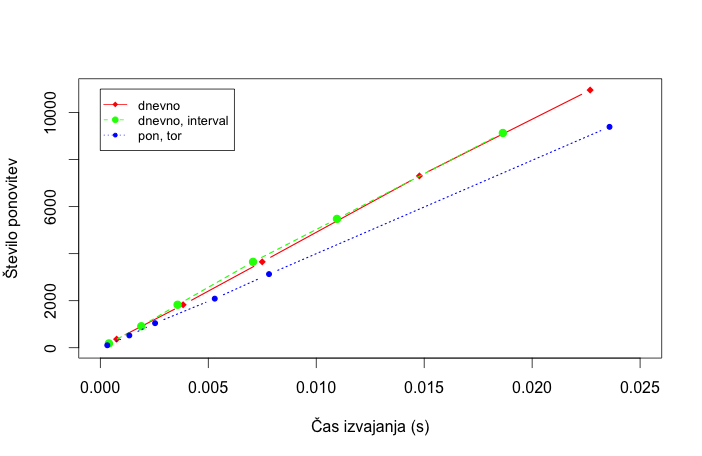
\includegraphics[width=\linewidth]{performance}
 \caption{Rezultati performančne analize C++ knjižnice.}
 \label{fig:performance}
\end{figure}

Kljub računski nezahtevnosti naše knjižnice si vseeno poglejmo kakšne posledice ima lahko vključitev C++ knjižnice v različne jezike, ki so v uporabi na izbranih platformah.

\subsection{Objective-C in C++}

Razlika v hitrosti izvajanja med kodo, napisano v jeziku C++, in Objective-C kodo je zanemarljiva, saj je Objective-C za platformo iOS domoroden jezik (\eng{native programming language}). Pri vključitvi C++ knjižnice v našo aplikacijo je moč zaznati malenkost višjo porabo pomnilnika (zaradi podvojenih objektov v C++ knjižnici), vendar za vse to poskrbimo v metodi \texttt{dealloc}, v kateri sprostimo pomnilnik.

Z zagotovostjo lahko trdimo, da vključitev C++ knjižnice v Objective-C projekt ne bo imel večjega vpliva na hitrost izvajanja aplikacije.

\subsection{Java in C++}

V raziskavi Univerze na Dunaju\cite{android-cpp} so ugotovili, da je Java s pomočjo \gls{jit} prevajalnika zmožna na preprostih primerih (recimo generiranje Fibonaccijevega zaporedja) v hitrosti izvajanja prehiteti C++ kodo. V nekoliko kompleksnejših primerih uporabe (recimo branje \gls{xml} dokumentov), kjer prevajalnik JIT ni bil zmožen pohitriti Java kode, pa je bil C++ vseeno hitrejši.

Avtorji na koncu navedejo, da vključevanje C++ kode v Android aplikacije ne bi smelo imeti velikega vpliva na hitrost, saj je bila hitrost izvajanje kode v večini primerov primerljiva.

\subsection{C\# in C++}

Za večino primerov je hitrost izvajanja C\# kode primerljiva izvajanju C++ kode. Razlike se začnejo kazati pri procesorsko zahtevnejših algoritmih, kjer se pokaže prednost C++ kode predvsem zaradi boljše izrabe pomnilnika\cite{windows-phone-dev}. Zavedati se moramo, da pri prevelikem prehajanju iz domorodne kode v C\# kodo lahko pride do izničenja vseh prednosti C++ kode, saj v vmesnem delu pride do pretvarjanja podatkovnih tipov iz C++ sveta v C\# svet (in obratno).

Po vsem tem lahko pridemo do istega zaključka kot v primeru Jave - vključitev C++ knjižnice v našo Windows Phone aplikacijo v večini primerov ne bo imelo prevelikega vpliva na hitrost.

\subsection{JavaScript in C++}

Na področju JavaScripta je bil v zadnjih nekaj letih videti velik napredek. S pomočjo asm.js\cite{asmjs}, ki je podmnožica jezika JavaScript, je spletnim brskalnikom v letu 2014 uspelo doseči le 2-kratno upočasnitev v primerjavi z domorodno kodo. Ista raziskava iz leta 2011 je pokazala kar 12-kratno upočasnitev\cite{html5-gamedev}.

Neposredno pisanje v asm.js je dokaj nerealno, saj razvijalca sili v pisanje kode na način, ki ga najbrž ni vajen (glej primer \ref{code:asm.js}). Namesto tega je asm.js še posebej primeren kot končni jezik za prevajanje med jeziki z ogrodjem, kot je Emscripten. Koda, prevedena iz jezika C++, bo zaradi tega v večini primerov hitrejša kot tista, ki jo razvijalec sam napiše v jeziku JavaScript.

\begin{lstlisting}[caption={Primer prevoda C kode v asm.js kodo.}, label=code:asm.js, language=JavaScript]
// C koda
int f(int i) {
  return i + 1;
}

// asm.js koda
function f(i) {
  i = i|0;
  return (i + 1)|0;
}
\end{lstlisting}


 








%==============================
\chapter{Conclusion}
\label{chap:conclusion}


 % use bibtex for bibliography









%==============================
\bibliographystyle{FRIthesis.sortbylastname}
\bibliography{thesis_bibliography}

 %% write your main thesis in logical individual chapters
% for better organization use a separate folder for images 
\graphicspath{{img/}}









%==============================
\appendix
\chapter{Appendix A}
\label{chap:a}


%-----
\section{Intro section}
All material unsuitable for the main part of the work (\eg~source code listings, extensive proofs, ...) should be placed in the Appendix.


%-----
\section{...}


\end{document}
